\section{Introduction}
The existence of search engine had changed the way people search 
for information, from exhaustively try to collect all different 
sources of information manually into an integrated searching experience, 
using a commercial search engine like Bing, Google, or Yahoo. 
It cannot be denied that search engine helps people to find information
easier. Every time we want to search about some particular information, 
we can simply enter our needs in the form of \textit{query} to a search 
engine. Over the years, improvements have been made on search engine to 
help users to form their query in a more correct way. One of this example 
is the query completion feature. User can enter something like 
``restaurant with'' in the search box and the search engine will provide 
the list of queries that contain ``restaurant with'', such as 
``restaurant with live music'' or ``restaurant with mariachi''. 
Table \ref{tab:querycompletion} shows the examples of query completion 
suggestion from Bing and Google. The query completion improves the user 
experience by helping user to form its query based on previously entered 
queries from other users who probably want to search for the same kind of 
information. 

\begin{table}[h]
\centering
\caption{Examples of query completion suggestion}
\begin{tabular}{ | p{3 cm} | p{3 cm} | }
\hline
\textbf{Bing} & \textbf{Google}\\ \hline
\textit{restaurant with} live jazz in baltimore md & \textit{restaurant with} with a view nyc \\ \hline 
\textit{restaurant with} live music & \textit{restaurant with} live music \\ \hline
\textit{restaurant with} games & \textit{restaurant with} mean girls menu \\ \hline
\textit{restaurant with} a view nyc & \textit{restaurant with} games \\ \hline
\textit{restaurant with} entertainment & \textit{restaurant with} private room \\ \hline
\end{tabular}
\centering
\label{tab:querycompletion}
\end{table}

Another exciting feature is the query spelling correction, which 
suggest the correct spelling of words when user mistype the query 
like ``estaurant in shanghai'' instead of ``restaurant in shanghai''. 
The search engine by default will look for the second form. Other 
additional feature might be in the form of list of suggestions of 
related search, that provides user with the related queries entered 
previously by other users that are considered related to current 
user query.

Apart from all this interesting and helpful features, most of the 
current commercial search engines are in nature a keyword-based 
search engine, that depend on the matches between words in user 
input query and words in web documents. This sometimes creates a 
problem for a novice user or a user who wants to search for certain 
information that he barely remembers or familiar with. Take for an 
example, a user who wants to search about a certain information about 
hurricane that hit one of the states in US some times ago, but by 
chance forget the name of the states. For some specific name or entity 
that is not clearly remembered, our mind works by first trying to 
grasp an \textit{abstraction} of that specific \textit{instance}, which 
in this case the \textit{concept} of a ``state'' and probably 
``hurricane''. But, what will happen when the user put the query 
like ``hurricanes in states'' is that, with high certainty, the 
results will not be exactly relevant to the user's need. The results 
may contain some web pages  with a list of hurricanes, which are not 
the \textit{exact} thing or name that the user wanted, as shown in 
Figure \ref{fig:exampleGoogleBing}.

\begin{figure}[h]
\centering
\includegraphics[scale=0.35]{images/hurricaneinstates-bing}
\includegraphics[scale=0.35]{images/hurricaneinstates-google}
\caption{Example of concepts and instances in Probase}
\label{fig:exampleGoogleBing}
\end{figure}

In this work, we focus on solving this specific problem. Given 
a vague query that contains concepts, we will provide users with 
the list of queries that are more specific. Our approach is 
simple, given the query, we will replace each abstract concept 
found in this query into its most specific instance, providing 
the user with the specific name of the ``hurricanes'' or ``states''. 
For the example above, our system is able to return 
``hurricane katrina in florida'' or ``hurricane hugo in south carolina'', 
that may suggest users directly to search for this query, rather than 
click into the website that contains list of hurricane and look for 
what he wants one by one.

In order to enable such kind of \textit{instantiation} we utilize 
a knowledge base called Probase \cite{website:Probase}, which is a 
taxonomical knowledge base that contains the information of the 
relation of concepts and their instances represented in a tree 
structured manner. The knowledge base contains more that 2.7 millions 
of concepts and extracted from 1 billion web pages, that should be 
able to match the wide domain of human known concepts.

Providing user with many queries where each of them contains 
instances of concepts in user input query is not enough. As one 
concept in Probase might be instantiated into a lot of instances, 
the resulting queries will not be entirely valid or correct, 
according to the world or human knowledge. Take an example of 
``president commit burglary''. In Probase, ``obama'' is an instance
of concept ``president'', and replacing the ``president'' with 
``obama' will be correct according to the knowledge base. However, 
the resulting query ``obama commit burglary'' will, somehow, in 
human perception, not a valid replacement. Taking this problem 
into account, we take advantage of using query log to 
\textit{validate} our resulting instantiations. Instead of 
generating a lot of incorrect queries, we provide user with 
the queries from the query log that contains the instantiation 
of user input query. As the query log contains queries entered 
by previous users, the resulting query will be, in some sense, 
a valid suggestion. In order to filter out those queries that 
are not useful or wrong, such as mistyped query, we use the 
information of query frequency and the number of click-through 
for that query.

The contributions that we give through our work are: 
\begin{enumerate}
\item 
Improving user experience and indirectly extend the capability of 
keyword-based search engine to the area of concept-based search, 
through the use of query suggestions feature that provide the 
instantiation of concepts found in user query.
\item
We propose a framework that can be used as a foundation to provide 
a concept-based query suggestions, that utilizes a taxonomical 
knowledge base and query log.
\item
Provide analysis and large scale evaluation of the framework.
\end{enumerate}

The paper is structured starting with the introduction of the Probase 
in section 2. We continue with the explanation of our query 
suggestion framework in section 3 and section 4. The evaluation 
and discussion of our experiment will be presented in section 5. 
We also provide some related works in section 6, and the conclusion 
of our work in section 7.

\begin{figure*}
\centering
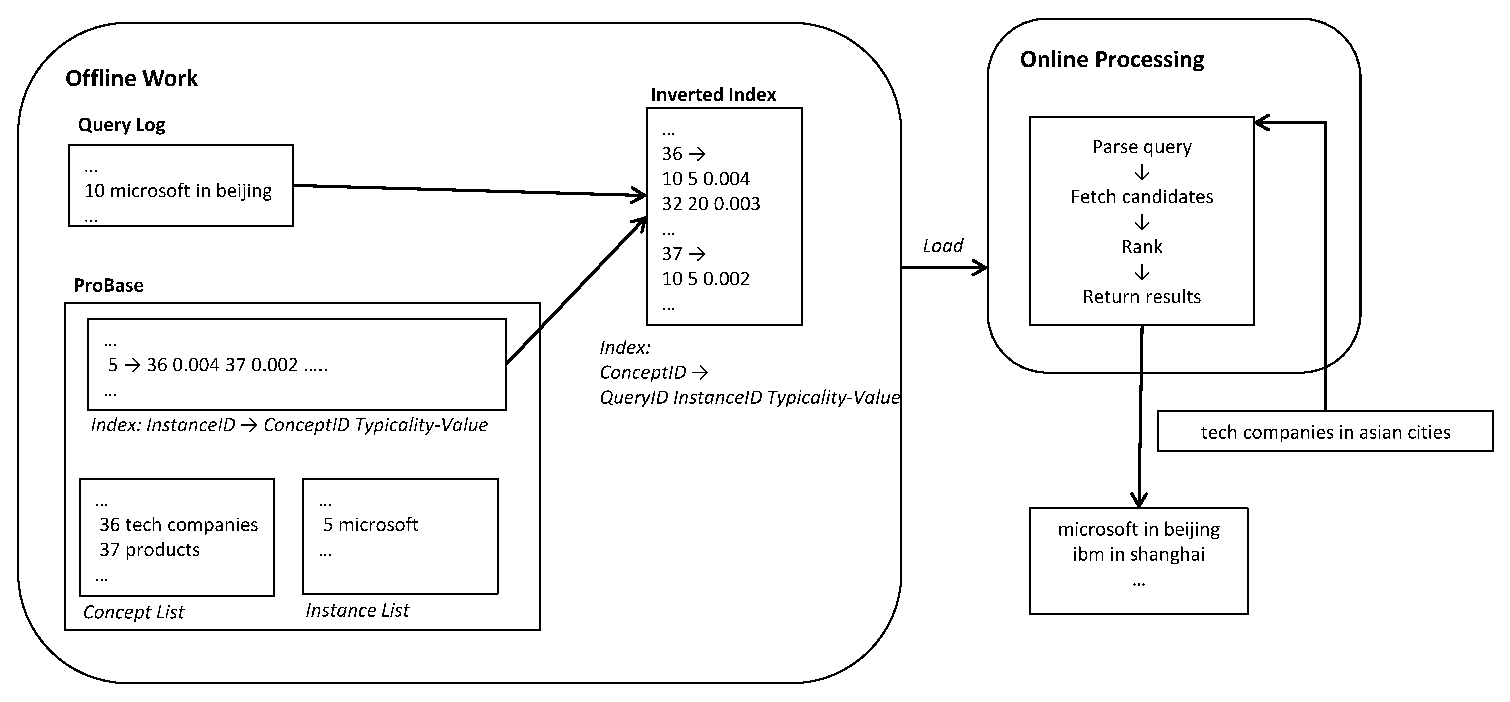
\includegraphics[scale=0.5]{images/Figure1}
\caption{Overview of the overall framework}
\label{fig:system}
\end{figure*}
